\documentclass[11pt,a4paper]{article}

\usepackage[margin=19mm,headheight=16pt,footskip=12mm]{geometry}
\usepackage{fontspec}
\setmainfont{Noto Serif}
\setsansfont{Inter}
\setmonofont{DejaVu Sans Mono}[Scale=0.86]
\usepackage{microtype}
\usepackage{parskip}
\usepackage{setspace}
\setstretch{1.05}

\usepackage{xcolor}
\definecolor{MMALSDark}{HTML}{1B1F23}
\definecolor{MMALSPanel}{HTML}{22272B}
\definecolor{MMALSInk}{HTML}{ECE7DD}
\definecolor{MMALSMuted}{HTML}{6F7A80}
\definecolor{MMALSLine}{HTML}{CBD1D5}
\definecolor{MMALSAmber}{HTML}{D98B21}
\definecolor{MMALSTeal}{HTML}{198F82}
\definecolor{MMALSBlue}{HTML}{3C78B5}
\definecolor{MMALSRed}{HTML}{B64B4B}
\definecolor{MMALSGreen}{HTML}{3A8E5D}
\definecolor{MMALSLight}{HTML}{F4F2ED}
\definecolor{MMALSCode}{HTML}{F6F7F8}

\usepackage{graphicx}
\usepackage{tikz}
\usetikzlibrary{arrows.meta,positioning,calc,fit,shapes.geometric,backgrounds}
\usepackage{booktabs}
\usepackage{tabularx}
\usepackage{longtable}
\usepackage{array}
\usepackage{multirow}
\usepackage{enumitem}
\setlist[itemize]{leftmargin=5.2mm,itemsep=1.7pt,topsep=3pt}
\setlist[enumerate]{leftmargin=6.2mm,itemsep=2pt,topsep=3pt}
\usepackage{amsmath,amssymb}
\usepackage{siunitx}
\usepackage{listings}
\usepackage[most]{tcolorbox}
\usepackage{hyperref}
\hypersetup{
  colorlinks=true,
  linkcolor=MMALSTeal,
  urlcolor=MMALSBlue,
  citecolor=MMALSTeal,
  pdftitle={MMALS Route-Function Activity Replay v0.1.1 User Manual},
  pdfauthor={MMALS Research Program},
  pdfsubject={User manual for the MMALS Activity Replay interactive viewer},
  pdfkeywords={MMALS, continual learning, route-function memory, activity replay, audit, geometry}
}
\usepackage{bookmark}
\usepackage{fancyhdr}
\usepackage{lastpage}
\usepackage{titlesec}
\usepackage{etoolbox}
\usepackage{needspace}
\usepackage{fontawesome5}

\pagestyle{fancy}
\fancyhf{}
\fancyhead[L]{\sffamily\small MMALS Activity Replay v0.1.1}
\fancyhead[R]{\sffamily\small User Manual}
\fancyfoot[L]{\sffamily\scriptsize MMALS Research Program}
\fancyfoot[R]{\sffamily\scriptsize Page \thepage\ of \pageref{LastPage}}
\renewcommand{\headrulewidth}{0.3pt}
\renewcommand{\footrulewidth}{0pt}

\titleformat{\section}{\sffamily\Large\bfseries\color{MMALSDark}}{\thesection}{0.7em}{}
\titleformat{\subsection}{\sffamily\large\bfseries\color{MMALSTeal}}{\thesubsection}{0.7em}{}
\titleformat{\subsubsection}{\sffamily\normalsize\bfseries\color{MMALSAmber}}{\thesubsubsection}{0.7em}{}
\titlespacing*{\section}{0pt}{15pt}{7pt}
\titlespacing*{\subsection}{0pt}{11pt}{5pt}
\titlespacing*{\subsubsection}{0pt}{8pt}{3pt}

\newcommand{\product}{\textsf{MMALS Route--Function Activity Replay}}
\newcommand{\version}{0.1.1}
\newcommand{\ui}[1]{\textsf{\bfseries #1}}
\newcommand{\code}[1]{\texttt{#1}}
\newcommand{\good}{\textcolor{MMALSGreen}{\faCheckCircle}}
\newcommand{\warn}{\textcolor{MMALSAmber}{\faExclamationTriangle}}
\newcommand{\infoicon}{\textcolor{MMALSBlue}{\faInfoCircle}}
\newcommand{\localicon}{\textcolor{MMALSTeal}{\faLaptop}}

\newcolumntype{Y}{>{\raggedright\arraybackslash}X}
\newcolumntype{P}[1]{>{\raggedright\arraybackslash}p{#1}}

\newtcolorbox{keybox}[1][]{
  enhanced, breakable, colback=MMALSLight, colframe=MMALSTeal,
  boxrule=0.7pt, arc=2mm, left=3mm,right=3mm,top=2.2mm,bottom=2.2mm,
  title=#1, fonttitle=\sffamily\bfseries, coltitle=MMALSDark
}
\newtcolorbox{warningbox}[1][]{
  enhanced, breakable, colback=MMALSAmber!7, colframe=MMALSAmber,
  boxrule=0.7pt, arc=2mm, left=3mm,right=3mm,top=2.2mm,bottom=2.2mm,
  title=#1, fonttitle=\sffamily\bfseries, coltitle=MMALSDark
}
\newtcolorbox{sciencebox}[1][]{
  enhanced, breakable, colback=MMALSBlue!5, colframe=MMALSBlue,
  boxrule=0.7pt, arc=2mm, left=3mm,right=3mm,top=2.2mm,bottom=2.2mm,
  title=#1, fonttitle=\sffamily\bfseries, coltitle=MMALSDark
}
\newtcolorbox{procedurebox}[1][]{
  enhanced, breakable, colback=white, colframe=MMALSLine,
  boxrule=0.7pt, arc=2mm, left=3mm,right=3mm,top=2.2mm,bottom=2.2mm,
  title=#1, fonttitle=\sffamily\bfseries, coltitle=MMALSDark
}

\lstdefinestyle{mmals}{
  basicstyle=\ttfamily\small,
  backgroundcolor=\color{MMALSCode},
  frame=single,
  rulecolor=\color{MMALSLine},
  framesep=5pt,
  breaklines=true,
  columns=fullflexible,
  showstringspaces=false,
  keywordstyle=\color{MMALSBlue}\bfseries,
  commentstyle=\color{MMALSMuted},
  stringstyle=\color{MMALSTeal}
}
\lstset{style=mmals}

\begin{document}

% -----------------------------------------------------------------------------
% Cover
% -----------------------------------------------------------------------------
\begin{titlepage}
\pagecolor{MMALSDark}\color{MMALSInk}

\begin{tikzpicture}[remember picture,overlay]
  \fill[MMALSTeal!18] (current page.south west) rectangle ([xshift=22mm]current page.north west);
  \fill[MMALSAmber] ([xshift=22mm]current page.south west) rectangle ([xshift=24mm]current page.north west);
  \draw[MMALSTeal!55,line width=1.1pt]
    ([xshift=32mm,yshift=-42mm]current page.north west)
    .. controls +(28mm,-12mm) and +(-28mm,15mm) .. ([xshift=-28mm,yshift=45mm]current page.south east);
  \draw[MMALSAmber!60,line width=0.7pt]
    ([xshift=42mm,yshift=-55mm]current page.north west)
    .. controls +(33mm,-6mm) and +(-25mm,10mm) .. ([xshift=-37mm,yshift=58mm]current page.south east);
\end{tikzpicture}

\vspace*{22mm}
\hspace*{13mm}\begin{minipage}{0.78\textwidth}
{\sffamily\bfseries\fontsize{13}{15}\selectfont\color{MMALSTeal} MMALS RESEARCH PROGRAM}\par
\vspace{8mm}
{\sffamily\bfseries\fontsize{34}{39}\selectfont Route--Function\par Activity Replay}\par
\vspace{5mm}
{\sffamily\fontsize{20}{24}\selectfont User Manual}\par
\vspace{11mm}
{\large Interactive training, inference, geometry, and scientific-audit viewer}\par
\vspace{15mm}
\begin{tcolorbox}[colback=MMALSPanel,colframe=MMALSLine!40,boxrule=0.6pt,arc=2mm,left=4mm,right=4mm,top=3mm,bottom=3mm]
\color{MMALSInk}\sffamily
\begin{tabularx}{\linewidth}{@{}P{34mm}Y@{}}
Product version & \version\\
Manual version & 1.0\\
Document date & 18 June 2026\\
Status & Operational guide for the standalone HTML prototype\\
\end{tabularx}
\end{tcolorbox}
\vfill
{\small\color{MMALSInk!75}
This manual describes the publish-ready repository and standalone viewer at\par
\code{github.com/gharbonnier78/mmals-activity-replay}.}
\end{minipage}
\end{titlepage}
\nopagecolor\color{black}

% -----------------------------------------------------------------------------
% Front matter
% -----------------------------------------------------------------------------
\thispagestyle{plain}
\begin{keybox}[At a glance]
\product\ is a local, browser-based replay and audit tool for MMALS experiment traces. It synchronizes an ecosystem graph, a route-simplex view, metric cards, time-series traces, event details, and an A-to-B comparison. The embedded demonstration uses MMALS v0.9 CSV exports. Compatible CSV files can be loaded directly from the user's computer; the viewer does not upload them.
\end{keybox}

\begin{warningbox}[Scope boundary]
The viewer is an observational instrument. It visualizes logged measurements and clearly marked proxies. It does not retrain a model, recompute routes, establish causality, or convert routing entropy into physical carbon emissions unless explicit energy or carbon columns are present.
\end{warningbox}

\tableofcontents
\clearpage

% -----------------------------------------------------------------------------
\section{Purpose and Scope}

\subsection{What the viewer is for}

Use the viewer to replay two complementary forms of MMALS activity:

\begin{itemize}
  \item \textbf{Training activity}: task and total losses, routing entropy, dominance, mutualistic gain, route-memory loss, distillation loss, and latent-memory loss.
  \item \textbf{Inference and audit activity}: retained-task accuracy, route allocation, route drift, latent functional drift, output drift, and checkpoint-to-checkpoint changes.
\end{itemize}

The synchronized interface helps answer practical questions such as:

\begin{itemize}
  \item When did a route become specialized?
  \item Did the selected route remain stable while the mediated function drifted?
  \item Did accuracy remain stable even though internal geometry changed?
  \item Which hosts gained or lost routing weight between two checkpoints?
  \item Is a displayed ``carbon'' value physical, or only the historical entropy proxy?
  \item Is a regime-change value a calibrated detector output, or an uncalibrated visual diagnostic?
\end{itemize}

\subsection{Disciplined biological mapping}

The interface preserves the MMALS mapping used throughout the research program:

\begin{table}[h]
\centering
\begin{tabularx}{\textwidth}{@{}P{35mm}P{47mm}Y@{}}
\toprule
\textbf{Biological term} & \textbf{MMALS element} & \textbf{Meaning in the viewer}\\
\midrule
Host organism / tree & Host neural module & A specialized representation-producing component, shown as a distinct node.\\
Fungal system / mycelial medium & Router and host-specific transformation system & The active mediator that combines, transforms, and allocates host signals.\\
Mycorrhiza & Host--medium exchange relation & The edges between hosts and the fungal medium; not a separate host and not the medium itself.\\
Carbon cost & Routing or physical resource cost & Routing entropy by default; physical energy or CO$_2$e only when explicitly logged.\\
Phosphorus / nutrient gain & Mutualistic contribution signal & Logged mean/minimum gain where available; not automatically a causal per-host estimate.\\
\bottomrule
\end{tabularx}
\end{table}

\subsection{Why route geometry is a simplex, not a torus}

For $M$ hosts, route weights satisfy
\[
  r_i \ge 0, \qquad \sum_{i=1}^{M} r_i = 1.
\]
They therefore live on the probability simplex $\Delta^{M-1}$. The viewer projects the five-host simplex to a two-dimensional barycentric display. A torus would be structurally justified only if the source variables contained two independent periodic coordinates. It is not imposed merely because toroidal geometry appears in other biological or artificial systems.

\begin{sciencebox}[Interpretation rule]
Treat the route-simplex point as a compact visualization of \emph{allocation}. Do not treat its apparent two-dimensional distance as an exact metric on the full four-dimensional five-host simplex unless a specific projection and distance have been validated for that purpose.
\end{sciencebox}

% -----------------------------------------------------------------------------
\section{Package Contents and Requirements}

\subsection{Files in the prototype package}

\begin{longtable}{@{}P{55mm}P{108mm}@{}}
\toprule
\textbf{File} & \textbf{Purpose}\\
\midrule
\endfirsthead
\toprule
\textbf{File} & \textbf{Purpose}\\
\midrule
\endhead
\code{index.html} & Standalone interactive viewer and GitHub Pages entry point.\\
\code{README.md} & Brief package description, fidelity boundaries, and recognized CSV families.\\
\code{losses\_df.csv} & Training checkpoints and losses used by the embedded v0.9 demonstration.\\
\code{history\_df.csv} & Post-task accuracy, route entropy, and dominance history.\\
\code{routes\_df.csv} & Per-host route weights at logged checkpoints.\\
\code{drift\_df.csv} & Route, latent, and output drift diagnostics.\\
\code{task\_forgetting\_df.csv} & Best/final task accuracy and per-task forgetting.\\
\code{model\_diag.csv} & Model-level summary diagnostics.\\
\code{scorecard.csv} & Final accuracy, forgetting, variability, and parameter counts.\\
\code{mmals\_event\_trace\_schema.csv} & Recommended long-format schema for a future event-level activity movie.\\
\bottomrule
\end{longtable}

\subsection{System requirements}

\begin{itemize}
  \item A current desktop browser with JavaScript enabled: Chromium/Chrome, Microsoft Edge, Firefox, or Safari.
  \item No web server is required for normal use.
  \item No network connection is required after the file is available locally.
  \item Sufficient browser memory for the selected CSV set. Very large event traces should be pre-filtered or sampled.
\end{itemize}

\begin{keybox}[Local-data behavior]
CSV files selected with \ui{Load CSV files} are read by browser-side JavaScript. The prototype contains no upload function and sends no data to a remote service.
\end{keybox}

% -----------------------------------------------------------------------------
\section{Quick Start}

\begin{procedurebox}[First replay in five steps]
\begin{enumerate}
  \item Extract the GitHub repository package to a local folder.
  \item Open \code{index.html} in a modern browser.
  \item Leave \ui{Mode} set to \ui{Training activity} and select a model/policy and seed.
  \item Press \ui{Play}; adjust \ui{Playback speed} as needed.
  \item Move the time slider to any checkpoint and inspect the ecosystem graph, route geometry, metric cards, traces, and current-event table together.
\end{enumerate}
\end{procedurebox}

\subsection{Fast inference/audit workflow}

\begin{enumerate}
  \item Change \ui{Mode} to \ui{Inference / audit}.
  \item Select the observed model/policy and seed.
  \item Enable the trace buttons for \ui{accuracy}, \ui{route drift}, \ui{latent drift}, and \ui{output drift}.
  \item Move to a checkpoint of interest and press \ui{Pin current as A}.
  \item Move to a later checkpoint B and read the A-to-B delta panel.
\end{enumerate}

\begin{warningbox}[Do not infer causality from one replay]
An A-to-B change shows association within the selected trace. A causal objective, route-swap, or ablation claim requires a controlled intervention and a separately logged run or event identifier.
\end{warningbox}

% -----------------------------------------------------------------------------
\clearpage
\section{Interface Overview}

\subsection{Page map}

\begin{center}
\resizebox{0.86\textwidth}{!}{%
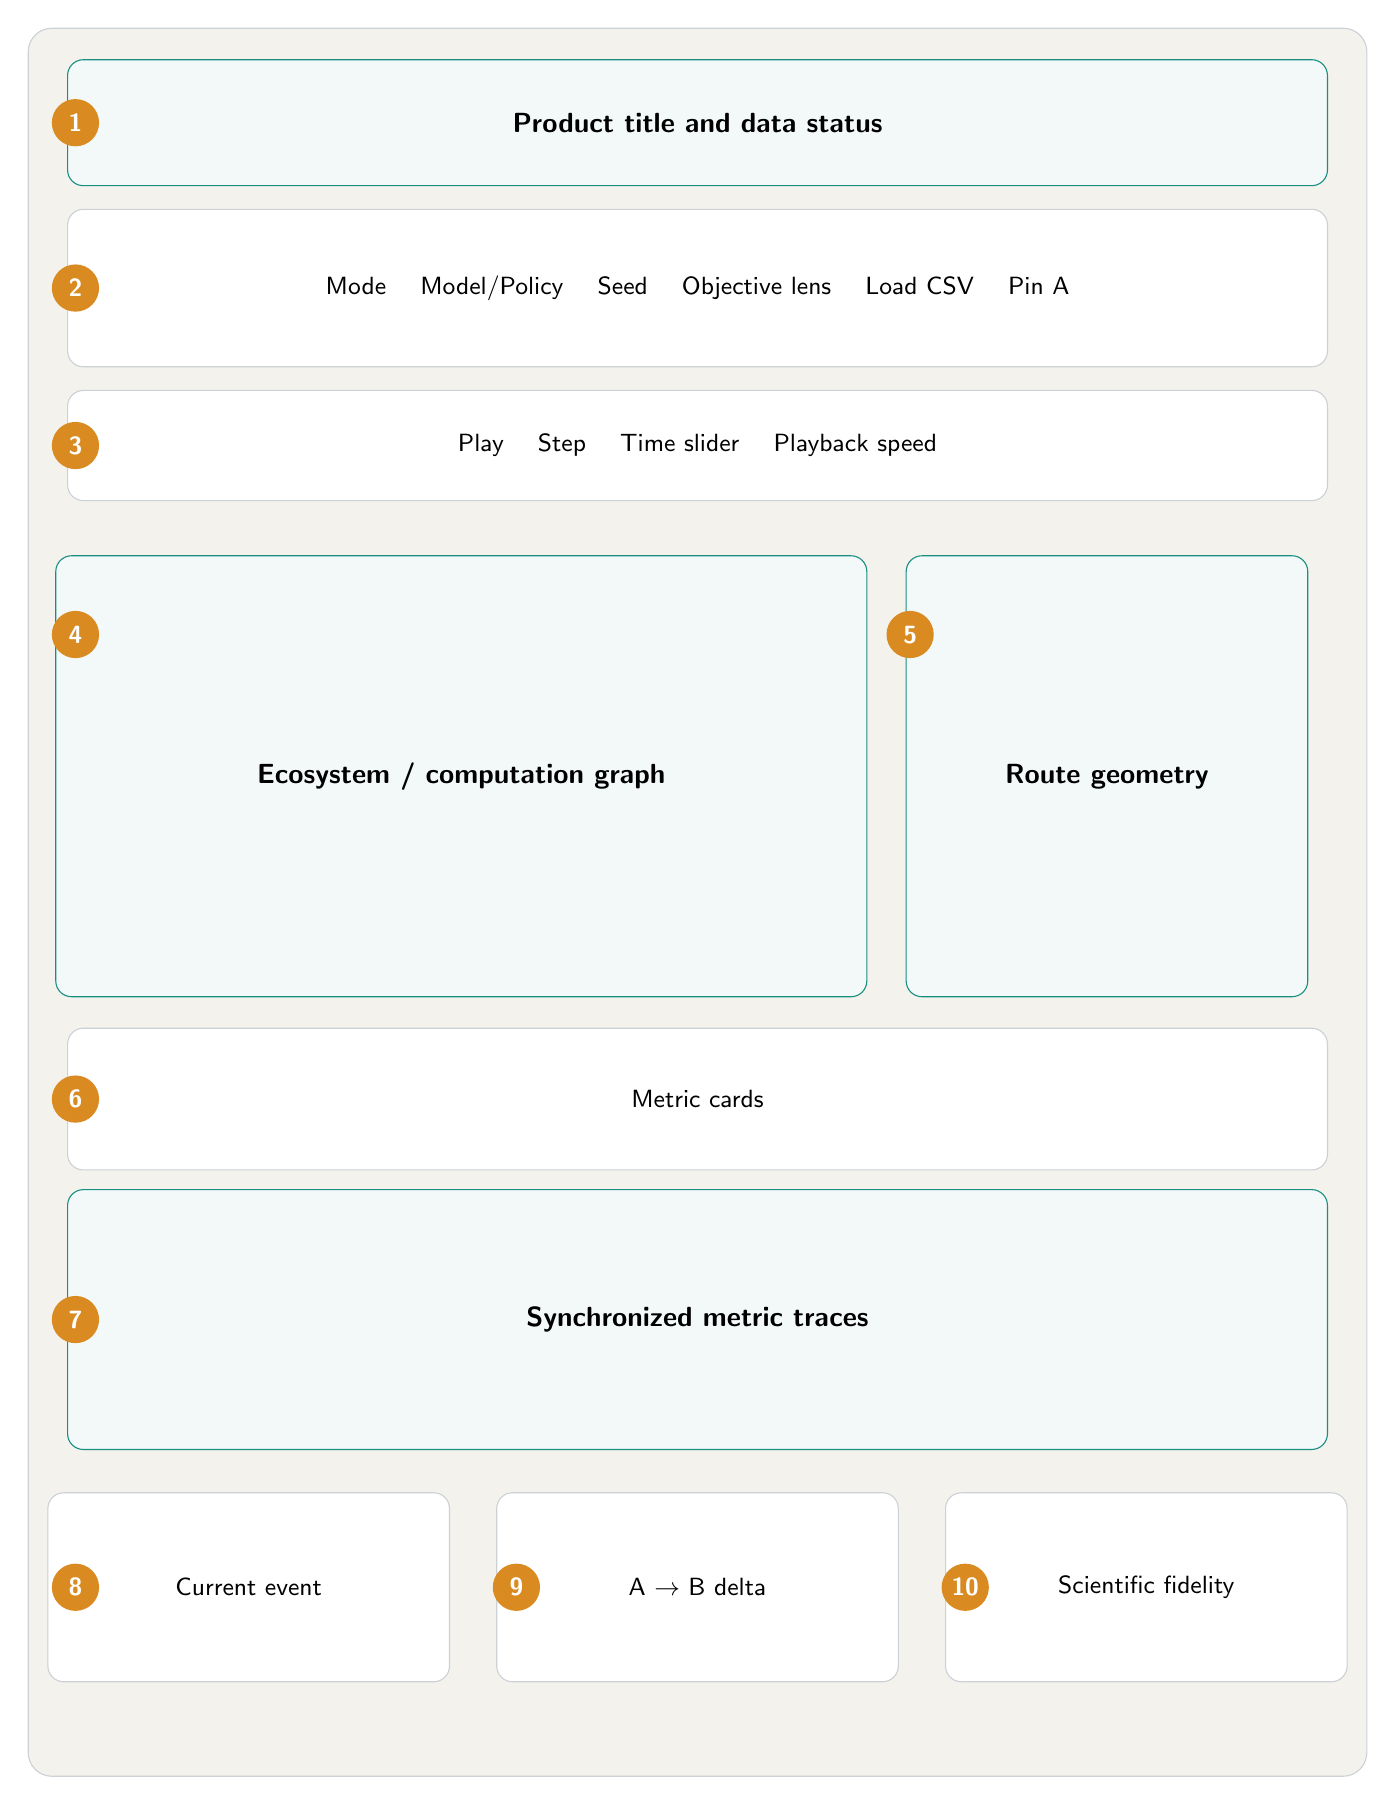
\begin{tikzpicture}[
  x=1mm,y=1mm,
  panel/.style={draw=MMALSLine,rounded corners=2mm,fill=white,minimum height=10mm,align=center,font=\sffamily\small},
  major/.style={draw=MMALSTeal,rounded corners=2mm,fill=MMALSTeal!5,align=center,font=\sffamily\bfseries},
  num/.style={circle,fill=MMALSAmber,text=white,minimum size=6mm,inner sep=0pt,font=\sffamily\bfseries\small}
]
  \draw[fill=MMALSLight,draw=MMALSLine,rounded corners=3mm] (0,0) rectangle (170,222);
  \node[major,minimum width=160mm,minimum height=16mm] at (85,210) {Product title and data status};
  \node[panel,minimum width=160mm,minimum height=20mm] at (85,189) {Mode \quad Model/Policy \quad Seed \quad Objective lens \quad Load CSV \quad Pin A};
  \node[panel,minimum width=160mm,minimum height=14mm] at (85,169) {Play \quad Step \quad Time slider \quad Playback speed};
  \node[major,minimum width=103mm,minimum height=56mm] at (55,127) {Ecosystem / computation graph};
  \node[major,minimum width=51mm,minimum height=56mm] at (137,127) {Route geometry};
  \node[panel,minimum width=160mm,minimum height=18mm] at (85,86) {Metric cards};
  \node[major,minimum width=160mm,minimum height=33mm] at (85,58) {Synchronized metric traces};
  \node[panel,minimum width=51mm,minimum height=24mm] at (28,24) {Current event};
  \node[panel,minimum width=51mm,minimum height=24mm] at (85,24) {A $\to$ B delta};
  \node[panel,minimum width=51mm,minimum height=24mm] at (142,24) {Scientific fidelity};
  \node[num] at (6,210) {1};
  \node[num] at (6,189) {2};
  \node[num] at (6,169) {3};
  \node[num] at (6,145) {4};
  \node[num] at (112,145) {5};
  \node[num] at (6,86) {6};
  \node[num] at (6,58) {7};
  \node[num] at (6,24) {8};
  \node[num] at (62,24) {9};
  \node[num] at (119,24) {10};
\end{tikzpicture}%
}
\refstepcounter{figure}
\par\smallskip
\begin{minipage}{0.90\textwidth}
\centering\small Figure \thefigure: Logical page map. All panels are synchronized to the same selected replay step.
\end{minipage}
\end{center}

\clearpage
\begin{longtable}{@{}P{12mm}P{45mm}P{96mm}@{}}
\toprule
\textbf{No.} & \textbf{Area} & \textbf{Function}\\
\midrule
\endfirsthead
\toprule
\textbf{No.} & \textbf{Area} & \textbf{Function}\\
\midrule
\endhead
1 & Header/status & Identifies the viewer and confirms whether the embedded demo or local files are active.\\
2 & Selection controls & Chooses mode, model/policy, seed, objective lens, data source, and A snapshot.\\
3 & Replay controls & Starts, pauses, steps, scrubs, and changes playback speed.\\
4 & Ecosystem graph & Displays component activity and forward/backward or memory relations using the MMALS biological mapping.\\
5 & Route geometry & Displays the current host-allocation point and its fading trail in a five-vertex simplex projection.\\
6 & Metric cards & Displays raw current values and a short statement about their source or proxy status.\\
7 & Synced traces & Displays selected normalized time-series lines aligned to the same playhead.\\
8 & Current event & Lists the active checkpoint's model, task, phase, route, losses, drifts, and related fields.\\
9 & A-to-B delta & Compares a pinned snapshot A with the current snapshot B.\\
10 & Scientific fidelity & States whether carbon, gain, regime, route time, and objective information are measured, approximated, or unavailable.\\
\bottomrule
\end{longtable}

% -----------------------------------------------------------------------------
\section{Controls}

\subsection{Mode}

\ui{Training activity} builds the replay primarily from a loss/checkpoint table containing fields such as \code{task\_id}, \code{epoch}, and \code{task\_loss}. It emphasizes training losses, route specialization, entropy, mutualistic gain, and memory terms.

\ui{Inference / audit} combines evaluation history, route checkpoints, and drift diagnostics. It emphasizes retained-task accuracy and internal drift after sequential learning.

\subsection{Observed model / policy}

The viewer constructs this list from the \code{model} or \code{method} column across recognized input tables. Changing the model rebuilds the replay and refreshes the available seeds.

\subsection{Seed}

The seed selector filters the selected model to one experimental realization. If the seed column is absent, the viewer treats the data as seed 0.

\subsection{Objective lens}

The objective lens changes visual emphasis and a composite display score. Available lenses are:

\begin{itemize}
  \item \ui{Balanced ecosystem}
  \item \ui{Performance}
  \item \ui{Stability}
  \item \ui{Mutualistic ecology}
  \item \ui{Efficiency / carbon}
\end{itemize}

\begin{warningbox}[Lens is not intervention]
Changing the lens does not recompute the route, model output, or training objective. It only changes how the already observed state is visually emphasized. Real objective-change analysis requires separate logged runs identified by \code{objective\_id} or an explicit goal vector.
\end{warningbox}

\subsection{Load CSV files}

Select one or several compatible CSV files. The viewer classifies files by their columns rather than by exact filename. The newly selected files replace the embedded dataset for the current browser session.

\subsection{Pin current as A}

Press this button to store the current state as comparison snapshot A. Continue the replay or move the slider to another state B. The A-to-B panel then displays deltas in available metrics and route weights.

\subsection{Play, Step, time slider, and speed}

\begin{table}[h]
\centering
\begin{tabularx}{\textwidth}{@{}P{37mm}Y@{}}
\toprule
\textbf{Control} & \textbf{Behavior}\\
\midrule
\ui{Play / Pause} & Advances through the ordered states or pauses at the current state.\\
\ui{Step} & Advances by one logged state. Useful for checkpoint-level inspection.\\
Time slider & Jumps directly to a replay index. All views update together.\\
Playback speed & Changes the delay between states from approximately $0.25\times$ to $8\times$. It does not alter the underlying timestamps.\\
\bottomrule
\end{tabularx}
\end{table}

% -----------------------------------------------------------------------------
\section{Main Visual Views}

\subsection{Ecosystem / computation graph}

The graph provides a stable component topology while metric values vary over time.

\begin{figure}[h]
\centering
\resizebox{\textwidth}{!}{%
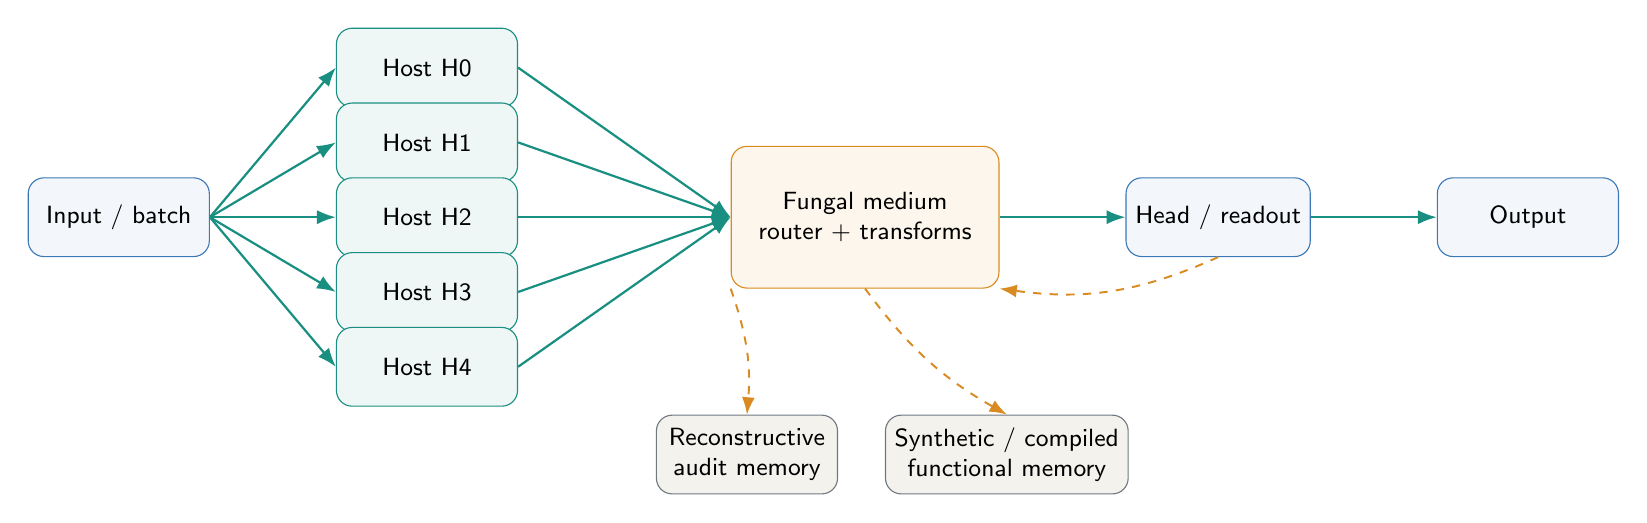
\begin{tikzpicture}[
  node distance=7mm and 16mm,
  box/.style={draw,rounded corners=2mm,minimum width=23mm,minimum height=10mm,align=center,font=\sffamily\small},
  host/.style={box,draw=MMALSTeal,fill=MMALSTeal!7},
  fungal/.style={box,draw=MMALSAmber,fill=MMALSAmber!8,minimum width=34mm,minimum height=18mm},
  other/.style={box,draw=MMALSBlue,fill=MMALSBlue!6},
  mem/.style={box,draw=MMALSMuted,fill=MMALSLight},
  fwd/.style={-{Latex[length=2.4mm]},line width=0.8pt,draw=MMALSTeal},
  back/.style={-{Latex[length=2.2mm]},line width=0.7pt,dashed,draw=MMALSAmber}
]
  \node[other] (input) {Input / batch};
  \node[host,right=of input,yshift=19mm] (h0) {Host H0};
  \node[host,right=of input,yshift=9.5mm] (h1) {Host H1};
  \node[host,right=of input] (h2) {Host H2};
  \node[host,right=of input,yshift=-9.5mm] (h3) {Host H3};
  \node[host,right=of input,yshift=-19mm] (h4) {Host H4};
  \node[fungal,right=27mm of h2] (fungal) {Fungal medium\\router + transforms};
  \node[other,right=of fungal] (head) {Head / readout};
  \node[other,right=of head] (out) {Output};
  \node[mem,below=16mm of fungal,xshift=-15mm] (audit) {Reconstructive\\audit memory};
  \node[mem,below=16mm of fungal,xshift=18mm] (synth) {Synthetic / compiled\\functional memory};
  \foreach \h in {h0,h1,h2,h3,h4}{\draw[fwd] (input.east) -- (\h.west); \draw[fwd] (\h.east) -- (fungal.west);}
  \draw[fwd] (fungal) -- (head);
  \draw[fwd] (head) -- (out);
  \draw[back] (head.south) to[bend left=16] (fungal.south east);
  \draw[back] (fungal.south west) to[bend left=12] (audit.north);
  \draw[back] (fungal.south) to[bend right=12] (synth.north);
\end{tikzpicture}%
}
\caption{Conceptual ecosystem graph used to interpret the replay.}
\end{figure}

Typical visual encodings include:

\begin{itemize}
  \item host node intensity or size: current route allocation and available gain signal;
  \item edge thickness: relative exchange strength;
  \item direction/style: forward activity, backward learning, or memory read/write;
  \item fungal-medium activity: mediated route/function state;
  \item objective node: display-lens score, not a causal change to the observed run.
\end{itemize}

\subsection{Route geometry}

For five hosts, the current route is a vector
\[
  r = (r_0,r_1,r_2,r_3,r_4), \qquad r_i\ge 0, \qquad \sum_i r_i=1.
\]
The viewer maps each host to one vertex of a regular pentagon and places the route point at the weighted average of the vertices.

\begin{figure}[h]
\centering
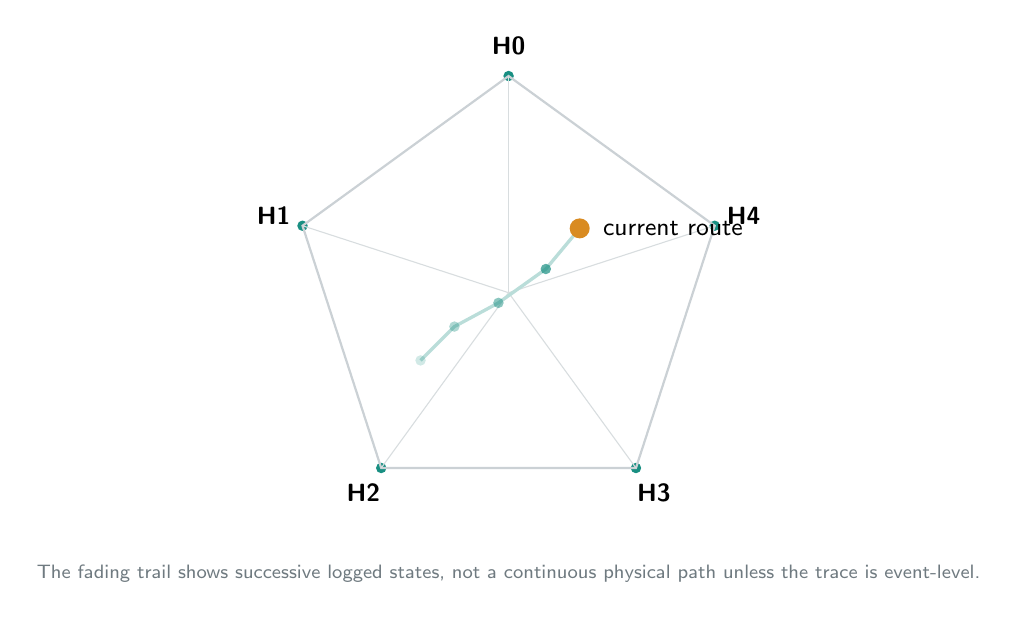
\begin{tikzpicture}[scale=0.86]
  \coordinate (C) at (0,0);
  \foreach \i/\lab in {0/H0,1/H1,2/H2,3/H3,4/H4}{
    \coordinate (V\i) at ({90+72*\i}:3.2);
    \fill[MMALSTeal] (V\i) circle (2.2pt);
    \node[font=\sffamily\bfseries\small] at ({90+72*\i}:3.65) {\lab};
  }
  \draw[MMALSLine,line width=0.8pt] (V0)--(V1)--(V2)--(V3)--(V4)--cycle;
  \foreach \i in {0,...,4}{\draw[MMALSLine!75] (C)--(V\i);}
  \draw[MMALSTeal!30,line width=1.2pt] (-1.3,-1.0) -- (-0.8,-0.5) -- (-0.15,-0.15) -- (0.55,0.35) -- (1.05,0.95);
  \foreach \x/\y/\o in {-1.3/-1.0/20,-0.8/-0.5/35,-0.15/-0.15/50,0.55/0.35/70}{\fill[MMALSTeal,opacity=\o/100] (\x,\y) circle (2.2pt);}
  \fill[MMALSAmber] (1.05,0.95) circle (4.2pt);
  \node[font=\sffamily\small,anchor=west] at (1.25,0.95) {current route};
  \node[font=\sffamily\scriptsize,text=MMALSMuted,align=center] at (0,-4.15) {The fading trail shows successive logged states, not a continuous physical path unless the trace is event-level.};
\end{tikzpicture}
\caption{Five-host route projection with a fading replay trail.}
\end{figure}

A point close to a vertex indicates strong routing dominance by that host. A point near the center indicates a more diffuse allocation. The trail helps reveal route movement, but checkpoint spacing may be uneven.

\subsection{Metric cards}

Cards show raw current values, usually including:

\begin{itemize}
  \item task loss or accuracy;
  \item route dominance;
  \item carbon / entropy;
  \item phosphorus / mutualistic gain;
  \item route, latent, or output drift;
  \item regime-change probability or proxy.
\end{itemize}

The explanatory text below each value is as important as the value itself. It identifies whether the metric was logged directly, derived from an available field, or substituted by a proxy.

\subsection{Synchronized traces}

Trace buttons turn individual metrics on or off. Each active line is normalized within the selected model/seed replay so that metrics with different units can share one chart. Raw values remain in cards and tooltips.

\begin{warningbox}[Normalization boundary]
Do not compare the vertical amplitude of two normalized lines as if their original units were identical. Use normalized traces to compare timing and direction; use cards, event tables, or exported CSV values for quantitative comparisons.
\end{warningbox}

\subsection{Current event}

The event table exposes the selected replay state's underlying values. It is the preferred place to confirm task identifiers, after-task index, epoch, phase, route status, and raw drift or loss fields.

\subsection{A-to-B delta}

After snapshot A is pinned, the panel compares A with the current state B. Available deltas include loss, accuracy, carbon/entropy, gain, and host route weights. A positive route delta means a host received more weight at B; a negative value means less.

\subsection{Scientific fidelity panel}

This panel is designed to prevent attractive graphics from becoming stronger scientific claims than the data support. It reports the status of:

\begin{itemize}
  \item carbon/energy measurement;
  \item phosphorus or mutualistic gain;
  \item regime-change probability;
  \item route timing and interpolation;
  \item objective changes.
\end{itemize}

% -----------------------------------------------------------------------------
\section{Training Replay Workflow}

\begin{procedurebox}[Recommended training inspection]
\begin{enumerate}
  \item Select \ui{Training activity}, model/policy, and seed.
  \item Start with \ui{task loss}, \ui{carbon / entropy}, \ui{phosphorus gain}, and \ui{regime change} traces active.
  \item Step through the first task and note when route dominance increases and entropy decreases.
  \item At each task boundary, inspect whether the route point moves abruptly or gradually.
  \item Enable memory-related traces or inspect the event table for route-memory, distillation, and latent losses.
  \item Pin A before an expected transition, move to B after the transition, and compare route allocation and losses.
\end{enumerate}
\end{procedurebox}

\subsection{How to read common training metrics}

\begin{longtable}{@{}P{38mm}P{42mm}P{77mm}@{}}
\toprule
\textbf{Metric} & \textbf{Typical field} & \textbf{Interpretation}\\
\midrule
\endfirsthead
\toprule
\textbf{Metric} & \textbf{Typical field} & \textbf{Interpretation}\\
\midrule
\endhead
Task loss & \code{task\_loss} & Supervised loss for the current task or batch checkpoint. Lower is usually better within a comparable run.\\
Total loss & \code{total\_loss} & Task loss plus active MMALS regularization/memory terms. It should not be compared directly across methods with different objectives without decomposition.\\
Entropy / carbon proxy & \code{entropy} or \code{route\_entropy} & Diffuseness of route allocation. Lower entropy means more concentrated routing, not automatically lower physical energy.\\
Dominance & \code{dominance} or \code{route\_dominance} & Maximum route weight. High dominance indicates concentrated allocation, but not necessarily useful specialization.\\
Mutualistic gain & \code{gain\_mean}, \code{gain\_min} & Aggregate contribution signal. A positive mean may coexist with a negative minimum. Per-host causality requires host-level ablation or gain fields.\\
Route-memory loss & \code{route\_memory\_loss} & Penalty for changing preserved route patterns. Low route drift does not guarantee low functional drift.\\
Distillation loss & \code{distill\_loss} & Difference between current and stored output behavior.\\
Latent loss & \code{latent\_loss} & Difference between current and stored mediated latent function.\\
Warm-up coefficient & \code{alpha} & Activation/ramp factor for delayed mutualistic or memory terms in compatible notebooks.\\
\bottomrule
\end{longtable}

\subsection{A useful diagnostic pattern}

A stable route with rising latent drift is important:
\[
  D_r \approx 0 \quad \text{while} \quad D_z > 0.
\]
It means the route identity remained similar while the computation through the route changed. This is a central route--function distinction in MMALS and is exactly the kind of pattern the viewer is intended to expose.

% -----------------------------------------------------------------------------
\section{Inference and Audit Replay Workflow}

\begin{procedurebox}[Recommended inference/audit inspection]
\begin{enumerate}
  \item Select \ui{Inference / audit}.
  \item Activate \ui{accuracy}, \ui{dominance}, \ui{latent drift}, and \ui{regime change} traces.
  \item Move through each \code{after\_task} checkpoint.
  \item Check whether old-task accuracy changes after later tasks are learned.
  \item Compare route drift $D_r$, latent drift $D_z$, and output drift $D_y$ rather than reading only final accuracy.
  \item Pin a pre-change state A and compare it with a later state B.
\end{enumerate}
\end{procedurebox}

\subsection{Drift hierarchy}

The prototype supports three complementary drift families:

\begin{align*}
D_r &= \mathbb{E}\,\lVert r_{\mathrm{current}}-r_{\mathrm{reference}}\rVert_2^2,\\
D_z &= \mathbb{E}\,\lVert z_{f,\mathrm{current}}-z_{f,\mathrm{reference}}\rVert_2^2,\\
D_y &= \mathbb{E}\,D_{\mathrm{KL}}\!\left(p_{\mathrm{reference}}\,\Vert\,p_{\mathrm{current}}\right).
\end{align*}

\begin{table}[h]
\centering
\begin{tabularx}{\textwidth}{@{}P{24mm}P{48mm}Y@{}}
\toprule
\textbf{Drift} & \textbf{Question} & \textbf{Caution}\\
\midrule
$D_r$ & Did host allocation change? & Route stability can be cosmetic if host functions or transforms drift.\\
$D_z$ & Did the mediated latent computation change? & Latent distance depends on representation scale and alignment.\\
$D_y$ & Did observable predictive behavior change? & Output stability can hide internal reorganization and may be task/head dependent.\\
\bottomrule
\end{tabularx}
\end{table}

\subsection{Accuracy and forgetting}

The history table may contain post-task accuracy $A^{(s)}_\tau$: performance on task $\tau$ after learning through task $s$. Per-task forgetting is commonly summarized as
\[
  F_\tau = \max_{s\ge \tau} A^{(s)}_\tau - A^{(K)}_\tau.
\]
The viewer can display the checkpoints used to understand this value, but it does not replace the experiment's statistical aggregation across seeds.

% -----------------------------------------------------------------------------
\section{Metric Dictionary and Scientific Meaning}

\subsection{Route entropy and dominance}

For route $r$ over $M$ hosts,
\[
  H(r) = -\sum_{i=1}^{M} r_i\log(r_i+\varepsilon),
  \qquad
  \mathrm{dominance}(r)=\max_i r_i.
\]

Low entropy and high dominance indicate concentrated routing. They do not, by themselves, prove host specialization. Stronger evidence requires contribution gain, ablation impact, representation separation, route--function stability, and cross-seed reproducibility.

\subsection{Carbon}

The viewer uses the following precedence:

\begin{enumerate}
  \item an explicit recognized field such as \code{carbon\_cost}, \code{co2e\_g}, \code{energy\_j}, or \code{energy\_kwh};
  \item otherwise, routing entropy as the historical MMALS ``carbon tax'' proxy.
\end{enumerate}

\begin{warningbox}[Units must remain visible]
An energy value in joules, an energy value in kilowatt-hours, and a CO$_2$e value in grams are different quantities. The event-level schema keeps them in separate columns. Do not merge them into a single unlabeled ``carbon'' score for scientific reporting.
\end{warningbox}

\subsection{Phosphorus / mutualistic gain}

The demonstration recognizes \code{gain\_mean} and \code{gain\_min}. Conceptually, a host contribution can be estimated by removing host $i$ and comparing loss:
\[
  G_i = \mathcal{L}_{\text{without }i} - \mathcal{L}_{\text{full}}.
\]
A positive $G_i$ means removal made the loss worse, so the host contributed under that intervention. The current v0.9 dump does not contain a causal $G_i$ for every host at every event. Consequently, host glow is driven mainly by route allocation and aggregate gain, not by a complete per-host causal estimate.

\subsection{Regime-change display}

If \code{regime\_prob}, \code{regime\_change\_prob}, or \code{context\_change\_prob} is present, the viewer displays that value as a logged detector output.

Otherwise, it constructs an uncalibrated visual proxy from changes in route, loss, drift, and known task boundaries. The proxy is useful for locating possible transitions, not for claiming a calibrated probability.

\subsection{Composite objective score}

The ecosystem graph may display a lens-dependent score combining performance, stability, ecology, and efficiency signals. This score is a visualization aid. It is not a contractual evaluation metric unless the research protocol explicitly freezes its formula and thresholds.

% -----------------------------------------------------------------------------
\section{Loading Your Own CSV Data}

\subsection{General rules}

\begin{itemize}
  \item Select all related CSV files in one file-picker action.
  \item Column names, not filenames, determine how tables are classified.
  \item The model identifier may be named \code{model} or \code{method}.
  \item Empty cells and the text \code{NaN} are treated as missing values.
  \item Numeric text is converted to numbers when possible.
  \item The newly loaded set replaces the embedded set until the page is reloaded.
\end{itemize}

\subsection{Recognized notebook-style families}

\begin{longtable}{@{}P{34mm}P{60mm}P{63mm}@{}}
\toprule
\textbf{Family} & \textbf{Minimum identifying columns} & \textbf{Useful optional columns}\\
\midrule
\endfirsthead
\toprule
\textbf{Family} & \textbf{Minimum identifying columns} & \textbf{Useful optional columns}\\
\midrule
\endhead
Training losses & \code{task\_id}, \code{epoch}, \code{task\_loss} & \code{total\_loss}, \code{entropy}, \code{dominance}, \code{gain\_mean}, memory losses, \code{alpha}\\
Routes & one or more \code{host\_0}, \code{host\_1}, \ldots columns & \code{after\_task}, \code{task\_id}, \code{task\_name}\\
Evaluation history & \code{after\_task}, \code{task\_id}, \code{acc} & \code{route\_entropy}, \code{route\_dominance}\\
Drift diagnostics & \code{route\_drift}, \code{latent\_drift}, \code{output\_drift} & task and model identifiers\\
Newer drift names & \code{route\_drift\_Dr}, \code{latent\_drift\_Dz}, \code{output\_drift\_Dy} & transformation/Jacobian drift fields\\
Explicit regime & any supported regime-probability field & true/predicted regime labels\\
Physical cost & any explicit energy or CO$_2$e field & latency, active parameters, hardware metadata\\
\bottomrule
\end{longtable}

\subsection{Example: minimum training CSV}

\begin{lstlisting}[language={},caption={Minimal training replay table}]
seed,model,task_id,task_name,epoch,task_loss,total_loss,entropy,dominance
0,example_policy,0,0 vs 1,0,0.52,0.58,1.31,0.34
0,example_policy,0,0 vs 1,1,0.28,0.33,0.91,0.55
0,example_policy,1,2 vs 3,0,0.61,0.75,1.22,0.41
\end{lstlisting}

\subsection{Example: route CSV}

\begin{lstlisting}[language={},caption={Five-host route checkpoints}]
seed,model,after_task,task_id,task_name,host_0,host_1,host_2,host_3,host_4
0,example_policy,0,0,0 vs 1,0.62,0.08,0.12,0.10,0.08
0,example_policy,1,0,0 vs 1,0.58,0.07,0.16,0.11,0.08
\end{lstlisting}

\subsection{Data-preparation checks}

Before loading, verify:

\begin{itemize}
  \item route weights are numeric and preferably sum to approximately 1;
  \item task identifiers use consistent numeric types;
  \item model and seed labels are consistent across files;
  \item \code{after\_task} and \code{task\_id} mean the same thing in all tables;
  \item physical cost columns include units in their names;
  \item regime probabilities are bounded to $[0,1]$ and are actually calibrated if described as probabilities.
\end{itemize}

% -----------------------------------------------------------------------------
\section{A-to-B Comparison}

\subsection{Basic use}

\begin{enumerate}
  \item Navigate to the baseline checkpoint.
  \item Press \ui{Pin current as A}.
  \item Move to another replay state B.
  \item Read the delta summary and per-host route bars.
  \item Record the model, seed, task, and replay indices before using the comparison in a report.
\end{enumerate}

\subsection{Good use cases}

\begin{itemize}
  \item before versus after a task boundary;
  \item early versus late epoch of one task;
  \item an old task immediately after learning versus after later tasks;
  \item a low-entropy checkpoint versus a high-entropy checkpoint;
  \item a suspected regime transition versus a stable neighborhood.
\end{itemize}

\subsection{Invalid or misleading use cases}

\begin{itemize}
  \item comparing different objective lenses and calling the visual difference a causal intervention;
  \item comparing states from different models without separately selecting and exporting them;
  \item treating normalized chart height as a raw effect size;
  \item calling a route-weight increase ``host benefit'' without contribution or ablation evidence;
  \item treating the uncalibrated regime proxy as a probability estimate.
\end{itemize}

% -----------------------------------------------------------------------------
\section{Scientific Fidelity Boundaries}

\begin{longtable}{@{}P{36mm}P{127mm}@{}}
\toprule
\textbf{Boundary} & \textbf{Operational meaning}\\
\midrule
\endfirsthead
\toprule
\textbf{Boundary} & \textbf{Operational meaning}\\
\midrule
\endhead
Route time & v0.9 contains route checkpoints rather than every optimizer step. Training routes may be transparently interpolated between a uniform start and a logged checkpoint.\\
Carbon & Routing entropy is used unless explicit physical energy or CO$_2$e columns exist.\\
Phosphorus gain & Aggregate mean/minimum gain may be logged; per-host causal gain is not reconstructed from aggregate data.\\
Regime probability & A calibrated value is shown only when a recognized probability column exists. Otherwise the viewer labels its value as a change proxy.\\
Objective changes & Lens selection changes visual emphasis only. Counterfactual objective effects require separate experimental runs.\\
Simplex projection & The two-dimensional pentagonal display is a projection of a higher-dimensional route simplex, not a proof of intrinsic two-dimensional geometry.\\
Graph topology & The component graph is a stable explanatory layout. Node position is not automatically a learned embedding.\\
Color and glow & Visual intensity is an aid to attention, not an independent measurement.\\
\bottomrule
\end{longtable}

\begin{sciencebox}[Recommended statement for papers or demonstrations]
``The viewer is used as a synchronized exploratory and audit interface over logged MMALS traces. Quantitative claims are computed from exported data and protocol-defined metrics; visual encodings are not treated as independent evidence.''
\end{sciencebox}

% -----------------------------------------------------------------------------
\section{Troubleshooting}

\begin{longtable}{@{}P{44mm}P{119mm}@{}}
\toprule
\textbf{Symptom} & \textbf{Resolution}\\
\midrule
\endfirsthead
\toprule
\textbf{Symptom} & \textbf{Resolution}\\
\midrule
\endhead
Blank page or controls do not respond & Confirm JavaScript is enabled. Reopen the file in a current browser. Check the browser developer console for a syntax or memory error.\\
The browser blocks local behavior & Move the complete package to a normal local folder. As a fallback, start a local server in that folder with \code{python -m http.server 8000} and open \code{http://localhost:8000/index.html}.\\
Model selector is empty after loading & At least one recognized table must contain a \code{model} or \code{method} value and identifying metric columns. Confirm headers have no hidden characters.\\
Seed selector shows only 0 & The seed column is absent, empty, or every row uses seed 0.\\
No route geometry appears & Load a route table with numeric \code{host\_0}, \code{host\_1}, \ldots columns matching the selected model and seed.\\
Route weights look incorrect & Check that weights are nonnegative and correspond to the same host order in every file. The viewer normalizes available route weights for display.\\
Carbon card shows entropy & No supported explicit energy/carbon field was found. Add \code{energy\_j}, \code{energy\_kwh}, \code{co2e\_g}, or \code{carbon\_cost}.\\
Gain is missing & The selected state has no \code{gain\_mean}/\code{gain\_min} data. This is common in inference-only exports.\\
Regime value says ``change proxy'' & No supported logged probability field is present. Add a real detector output under a recognized column name.\\
Replay jumps between sparse checkpoints & The source table is checkpoint-level. Export event-level or more frequent state rows for smoother replay.\\
Page becomes slow with large files & Pre-filter by model/seed/task, down-sample high-frequency rows, or split event traces. The current prototype loads all selected rows into browser memory.\\
A-to-B panel seems inconsistent & Re-pin A after changing mode, model, seed, or data set. Those changes rebuild the replay state.\\
Normalized traces look flat & A metric may have little variation or only one non-missing value. Inspect raw cards/event values.\\
\bottomrule
\end{longtable}

% -----------------------------------------------------------------------------
\section{Recommended Event-Level Trace}

Notebook-style CSV dumps are sufficient for checkpoint replay. A true architecture-agnostic activity movie is better represented by a long-format event trace: one row per component or exchange event, globally ordered by \code{step}.

\subsection{Core event groups}

\begin{longtable}{@{}P{37mm}P{126mm}@{}}
\toprule
\textbf{Group} & \textbf{Recommended fields}\\
\midrule
\endfirsthead
\toprule
\textbf{Group} & \textbf{Recommended fields}\\
\midrule
\endhead
Ordering and time & \code{step}, \code{wall\_time\_s}, \code{mode}, \code{phase}\\
Experiment identity & \code{model}, \code{backbone}, \code{seed}, \code{objective\_id}, \code{task\_id}\\
Context/regime & \code{regime\_true}, \code{regime\_pred}, \code{regime\_prob}\\
Interaction & \code{src\_component}, \code{dst\_component}, \code{direction}, \code{signal\_type}, \code{exchange\_value}\\
Component state & \code{component\_activity}, \code{host\_id}, \code{route\_weight}\\
Specialization & \code{host\_gain}, \code{host\_ablation\_delta}, \code{route\_entropy}, \code{route\_dominance}\\
Performance and memory & \code{task\_loss}, \code{memory\_loss}, \code{accuracy}\\
Geometry and drift & \code{route\_drift}, \code{latent\_drift}, \code{output\_drift}, \code{transform\_drift}\\
Calibration & \code{calibration\_width}\\
Operational cost & \code{latency\_ms}, \code{active\_params}, \code{energy\_j}, \code{energy\_kwh}, \code{co2e\_g}\\
Legacy proxy & \code{carbon\_proxy\_entropy}\\
Provenance & \code{notes} plus run/commit/config identifiers in future extensions\\
\bottomrule
\end{longtable}

\subsection{Direction vocabulary}

Recommended controlled values include:

\begin{itemize}
  \item \code{forward}: activations or mediated signals moving toward prediction;
  \item \code{backward}: gradient or credit-assignment signals;
  \item \code{memory\_read}: retrieved reconstructive or compiled memory;
  \item \code{memory\_write}: creation/update of memory artifacts;
  \item \code{audit}: measurement-only events that do not affect model state.
\end{itemize}

\subsection{Architecture-independent components}

Component identifiers can cover MLPs, CNNs, transformer blocks, routers, heads, adapters, memories, and external tools. Examples:

\begin{lstlisting}[language={},caption={Example component identifiers}]
input.batch
encoder.cnn.block_2
encoder.transformer.layer_5.attention
host.0
host.3
fungal.router
fungal.transform.3
memory.reconstructive
memory.compiled
head.task_2
output.logits
\end{lstlisting}

% -----------------------------------------------------------------------------
\section{Suggested Research Workflows}

\subsection{Route--function gap audit}

\begin{enumerate}
  \item Select inference/audit mode.
  \item Trace $D_r$, $D_z$, $D_y$, and accuracy.
  \item Locate intervals with low $D_r$ but high $D_z$.
  \item Compare the same tasks and seeds across route-only and functional-memory methods outside the viewer using the exported data.
\end{enumerate}

\subsection{Host-specialization audit}

Use the viewer to locate candidate specialization events, then confirm them with:

\begin{itemize}
  \item route entropy and dominance;
  \item host contribution gain;
  \item host ablation delta;
  \item representation separation;
  \item route--function stability;
  \item candidate-permutation controls;
  \item cross-seed reproducibility.
\end{itemize}

\subsection{Regime-change detector audit}

\begin{enumerate}
  \item Export the detector's actual \code{regime\_prob}.
  \item Display it next to route, latent, output, and performance traces.
  \item Mark ground-truth regime boundaries separately.
  \item Evaluate calibration, detection delay, false alarms, and downstream action policy outside the visual replay.
\end{enumerate}

\subsection{Objective-change experiment}

To study a real objective intervention rather than a display lens:

\begin{enumerate}
  \item freeze the data split, host bank, initialization policy, and evaluation protocol;
  \item run each objective under a unique \code{objective\_id};
  \item log goal-vector values and all affected costs;
  \item compare routes, functions, host contribution, accuracy, forgetting, and operational cost across matched seeds;
  \item use the viewer to replay each run, then use protocol-defined statistics for the claim.
\end{enumerate}

% -----------------------------------------------------------------------------
\section{Frequently Asked Questions}

\subsection*{Does the viewer prove that MMALS works?}
No. It helps inspect and communicate experiment traces. Evidence comes from controlled protocols, correct baselines, repeated seeds, statistical analysis, and reproducible artifacts.

\subsection*{Why is there no torus view?}
The route is a simplex variable. A torus should be added only for genuinely periodic coordinates or validated toroidal latent structure.

\subsection*{Can it replay CNNs, transformers, routers, and heads?}
Yes, conceptually, when they are represented as component and exchange events. The current v0.1 notebook-style loader is optimized for MMALS checkpoint tables; the event-level schema is the path to generalization.

\subsection*{Does the efficiency lens change the selected route?}
No. It changes visual emphasis only.

\subsection*{Is routing entropy an estimate of CO$_2$ emissions?}
No. It is a model-level proxy for diffuse routing. Physical energy and CO$_2$e require explicit measurements and system-boundary documentation.

\subsection*{Does a glowing host mean it is causally useful?}
Not necessarily. In the current demonstration, glow is driven by route allocation and aggregate gain availability. Causal usefulness needs host-level intervention evidence.

\subsection*{Are local CSV files uploaded?}
No. They are parsed locally in the browser by the standalone page.

\subsection*{Can I use screenshots in a paper?}
Yes, as explanatory figures, provided the caption states that the graphic is a visualization of logged traces and identifies measured versus proxy values. Numerical claims should cite the underlying tables and protocol.

% -----------------------------------------------------------------------------
\appendix
\section{One-Page Operator Checklist}

\begin{keybox}[Before opening]
\begin{itemize}
  \item Extract the complete package.
  \item Keep related CSV files together.
  \item Confirm browser JavaScript is enabled.
\end{itemize}
\end{keybox}

\begin{keybox}[Before interpreting]
\begin{itemize}
  \item Confirm mode, model/policy, and seed.
  \item Read the scientific-fidelity panel.
  \item Check whether carbon and regime values are measured or proxies.
  \item Confirm whether the replay is checkpoint-level or event-level.
\end{itemize}
\end{keybox}

\begin{keybox}[Before comparing A and B]
\begin{itemize}
  \item Pin A after the correct replay rebuild.
  \item Record A and B step/task identifiers.
  \item Inspect raw values, not only normalized traces.
  \item Do not call a visual delta causal without an intervention.
\end{itemize}
\end{keybox}

\begin{keybox}[Before publishing]
\begin{itemize}
  \item Export and archive source CSVs, configuration, seed, and commit identifier.
  \item State proxy definitions and units.
  \item Validate claims across matched controls and seeds.
  \item Use the viewer as an audit/explanation layer, not as the sole evidence source.
\end{itemize}
\end{keybox}

\section{Color and Symbol Legend}

\begin{table}[h]
\centering
\begin{tabularx}{\textwidth}{@{}P{26mm}P{35mm}Y@{}}
\toprule
\textbf{Color/symbol} & \textbf{Typical use} & \textbf{Meaning}\\
\midrule
\textcolor{MMALSTeal}{\rule{12mm}{2mm}} Teal & Hosts, routes, forward exchange & Active allocation or mediated signal.\\
\textcolor{MMALSAmber}{\rule{12mm}{2mm}} Amber & Objective, warnings, current route & Attention, selected state, or cost-oriented signal.\\
\textcolor{MMALSBlue}{\rule{12mm}{2mm}} Blue & Outputs, information, audit aids & Readout, information, or explanatory status.\\
\good & Confirmed / available & Logged or operational state is available.\\
\warn & Warning / proxy & Interpretation requires a boundary or caveat.\\
\infoicon & Information & Explanatory or non-causal display element.\\
\bottomrule
\end{tabularx}
\end{table}

\section{Version Notes}

\begin{tabularx}{\textwidth}{@{}P{24mm}P{28mm}Y@{}}
\toprule
\textbf{Version} & \textbf{Date} & \textbf{Notes}\\
\midrule
Viewer 0.1.1 & June 2026 & Standalone HTML prototype; embedded v0.9 demonstration; training/inference modes; ecosystem graph; route-simplex geometry; synced traces; A-to-B comparison; local CSV loading; fidelity panel.\\
Manual 1.0 & 18 June 2026 & Initial operational manual covering controls, data schemas, metrics, scientific boundaries, troubleshooting, and future event-level trace.\\
\bottomrule
\end{tabularx}

\vfill
\begin{center}
{\sffamily\bfseries\color{MMALSTeal} End of manual}\par
\smallskip
{\small MMALS Route--Function Activity Replay v0.1.1}
\end{center}

\end{document}
